% !TEX encoding = UTF-8 Unicode
\documentclass[a4paper]{article}

\usepackage[utf8]{inputenc}
\usepackage[T1]{fontenc}
\usepackage{amsmath}
\usepackage{amsfonts}
\usepackage{graphicx}
\usepackage{xcolor}

\newcommand{\bs}[1]{{\color{blue}\textbackslash{}#1}}

\author{J.M. Pérez Pardo} %Declaring the author for the maketitle command
\title{A primer on \LaTeX} %Declaring the title for the maketitle command
\date{\today} %Declaring the date for the maketitle command. \today prints the current date. You can write anything, including things that are not a date. 

\begin{document}

\maketitle

\tableofcontents

\section{Introduction}

We are going to construct now a template or sample document which covers the main tools that one needs to produce a complex \LaTeX{} document. Most of the things that you will ever need and many more are covered throughly in \cite{MittelbachGoossens2004}. In the next lecture we are also going to cover some more advanced material to understand how the internals of \LaTeX{} work. This is rarely used directly but it helps to understand why \LaTeX{} does things the way it does and it saves time. All the details can be found in the book by the father of \TeX, D. Knuth \cite{Knuth1990}.

\section{The Preamble}

The very first four lines of your document should be the following. 

\begin{verbatim}
% !TEX encoding = UTF-8 Unicode
\documentclass...

\usepackage[utf8]{inputenc}
\usepackage[T1]{fontenc}


\end{verbatim}


The first line, including the comment, must be line 1 in the source file. These three lines together make unicode encoding and fonts work natively in the document. This way you do not need to care about special characters like é í ä ó. They will work as expected. 

The preamble is the place in the source file between these lines and the \bs{begin}\{document\} statement. All the packages to be used in a document should be called there. Check the preamble of the source file associated with this document to get an idea of its typical structure.

\section{Title and other headings}

The formatting of the title and other headings depends on the class, as many other things. They can be modified by redefining the corresponding macros. Typically the style and macros used to define the headings of the document depend on the journal or editorial where you will publish the document. The article class (as well as book and report) include a simple way of producing this heading. There are some macros like \bs{author}, \bs{title}, \bs{date} which then are transformed using the \bs{maketitle} command. In the article class the \bs{maketitle} needs to be included after the \bs{begin}\{document\} statement. The rest of the macros will go typically in the preamble. Check how they are used in the source file.


\section{Table of contents}

%\tableofcontents

\section{Mathematics in a Document}

\subsection{The math modes and the text mode}

Typesetting mathematics in a document was one of the reasons why \TeX{} and later \LaTeX{} was created. There are two types of math modes: inline mode and displayed mode. Inline mode is when an equation or mathematical expression is embedded in the text, $\sum_{j=1}^{n=10}x^j$, like this one. It is included in the source text with the symbol \$. A single \$ starts the inline math mode and another \$ ends it. Another way of inserting math in the inline mode is surrounding it with the symbols \textbackslash(, \textbackslash), like here  \(\lim_{x\to\infty} f(x) = 7\). The math mode and the text mode have many differences. For instance, regular latin characters are displayed in italics and spaces are ignored $This is math mode$. Display mode can be called using double dollar symbols \$\$,\$\$ or enclosing it with \textbackslash[, \textbackslash] like here $$\sum_{j=1}^{n=10}x^j$$ or \[\lim_{x\to\infty} f(x) = 7.\]

As opposed to inline math mode, the displayed mode prints the mathematical expression in a separated line. Wether this equation is centred, right aligned or left aligned depends on the class and styling. Notice that there are differences in how the math is typeset in the two modes. The inline mode is more compact and sub and superscripts are placed at different positions.

\subsection{Some environments useful for presenting equations}

\noindent {\bfseries The equation environment.}

It includes automatically a tag for the equation. Look at the number at the margin. The number can be associated to a label with the \bs{label} command. 

  \begin{equation}\label{my_equation}
    \int_{\infty}^\infty e^{-x^2} dx = \sqrt{\pi}
  \end{equation}

I can refer to point to the equation \ref{my_equation}.\\

\noindent {\bfseries The align environment.}

The following environments require the {\ttfamily amsmath} package. Is is loaded in the preamble. The align environment is useful to typeset many equations together. Each equation gets its own tag. You can prevent an equation from getting a tag by using the \bs{notag} command.
%
  \begin{align}
    (a+b)^2 &= a^2 + 2ab + b^2 \\
      & \geq 0 \\
      & > - x^2 +5 \notag
   \end{align}
%   
The starred version, \emph{align*}, produces the same ouput but introduces no tags.

  \begin{align*}
    (a+b)^2 &= a^2 + 2ab + b^2 \\
      & \geq 0 \\
      & > - x^2 +5
  \end{align*}
   
\subsection{Tabular math}

  Matrix-like environments use \bs{\bs{}} to separate rows and \& to separate columns. Different brackets can be chosen:
  
  %matrix, pmatrix, bmatrix,

  $$%
    A = %
    \begin{bmatrix}
      a & b \\ c & d
    \end{bmatrix} \neq %
    \begin{matrix}
      a & b \\ c & d
    \end{matrix} \neq %
    \begin{pmatrix}
      a & b \\ c & d
    \end{pmatrix}
  $$
%
Another common matrix-like environment is the \emph{cases} environment.

  $$
  f(x ) = %
    \begin{cases}
      \exp\left(-\frac{1}{x}\right) &, \text{if } x > 0 \\
      0 &, \text{if } x\leq 0
    \end{cases}
  $$


\section{Tables in text mode. The tabular environment}

One can produce tables in latex. We will speak about the basic functionality. The functionality can be extended by using packages that can be loaded in the preamble. There is a mandatory argument that specifies the alignment of each column. The pipe | in the argument determine wheter to split the adjacent columns by a vertical line.

\begin{tabular}{l c r | c} % Warning, small L is l and the pipe |. They are typeset very similar depending on the font of hte editor. Small L is for left alignment will the pipe is to include a vertical line between the columns.
Aligned lef & An Oak &  Aligned right & An Oak \\
$\emptyset$ & Centered & $\emptyset$ &  Centered \\
\hline %This command puts a horizontal line in the table
$\emptyset$ & $\emptyset$ & $\emptyset$ &  $\emptyset$ \\
\end{tabular}


\section{List environments}

\begin{itemize}
  \item First element
  \item Second element
\end{itemize}

\begin{enumerate}
  \item First element
  \item Second element
\end{enumerate}

\begin{enumerate}
  \item First element
    \begin{enumerate}
      \item element 1.1
      \begin{enumerate}
        \item element 1.1.1
        \item element 1.1.2
        \item element 1.1.3
      \end{enumerate}
      \item element 1.2
    \end{enumerate}
  \item Second element
\end{enumerate}

The labels of the nested enumerate environment can be changed. This is done with the special commands 
\bs{labelenumi}, \bs{labelenumii}, \bs{labelenumiii}, \bs{labelenumiv}, \bs{theenumi}, \bs{theenumii} and so on. The \texttt{i}'s determine the nesting level in roman numbers. Check the code to see how to change the labels.

\theenumii 

\theenumiii

\renewcommand\theenumii{\Roman{enumii}}

\theenumii

\begin{enumerate}
  \item First element
    \begin{enumerate}
      \item element 1.1
      \begin{enumerate}
        \item element 1.1.1
        \item element 1.1.2
        \item element 1.1.3
      \end{enumerate}
      \item element 1.2
    \end{enumerate}
  \item Second element
\end{enumerate}


\renewcommand\labelenumii{\theenumii]] ->}

\begin{enumerate}
  \item First element
    \begin{enumerate}
      \item element 1.1
      \begin{enumerate}
        \item element 1.1.1
        \item element 1.1.2
        \item element 1.1.3
      \end{enumerate}
      \item element 1.2
    \end{enumerate}
  \item Second element
\end{enumerate}

We will see more functionality of the command \bs{renewcommand}. This is very useful and a must-to-know for every \LaTeX{} user.

\section{Changing Fonts in a \LaTeX{} Document}

\begin{itemize}

\item Series 

  \begin{itemize}
    \item Bold; \textbf{I am Bold}; {\bfseries I am bold}

    \item Medium(default); \textmd{ I am normal}; {\mdseries I am normal} ; {\mdseries I am normal}

      \textbf{ This is bold \textmd{this is not} } 
  
  \end{itemize}

\item Family

  \begin{itemize} 
    \item Serif font (default); \textrm{Here am I }; {\rmfamily Here am I};

    \item Sans Serif font; \textsf{Here am I}; {\sffamily Here am I}
    
    \item Typewriter font; \texttt{text}; {\ttfamily Here am I }

  \end{itemize}

\item Shape

  \begin{itemize}
    \item upright (default); \textup{Normal}; {\upshape also normal}
    \item slanted/italics; \textit{I am in italics}; {\itshape Also in italics}
    \item small caps: \textsc{I am In Small Caps}; {\scshape i am Also}
  \end{itemize}

\end{itemize}

You can mix the three properties, some particular combinations might not be available: {Hello} {\ttfamily \itshape Hello} {\sffamily \itshape Hello} {\sffamily \bfseries Hello} {\bfseries Hello} {\ttfamily \bfseries Hello} {}

\section{Defining macros}

You can define your own macros. This is done with the following commands:\\

\noindent\bs{newcommand}\{\bs{newcommandname}\}\{code to be substituted when \bs{newcommandname} is written\}\\
\bs{renewcommand}\dots

The difference between them is that they check if a given command is already defined. To override an already defined command you need to use \bs{renewcommand}.

\noindent I will define the following macro:
\noindent \verb!\newcommand\R{\mathbb{R}}!\\

\noindent The \emph{mathbb} command requires the amsfonts package.\\
 
\newcommand\R{\mathbb{R}} %\mathbb requires the amsfonts package


$\R$

\noindent {\bfseries Commands with arguments}\\

The number of arguments is determined with square brackets. The arguments are called within the macro prepending a \#. Check the code.

\newcommand\average[1]{\langle#1\rangle}

$\average{A}$\\

\newcommand\fraction[2]{\frac{#1}{#2}}

$\fraction{\text{Numerator}}{\text{Denominator}}$\\


\section{Including Graphics}

\begin{figure}[h]
  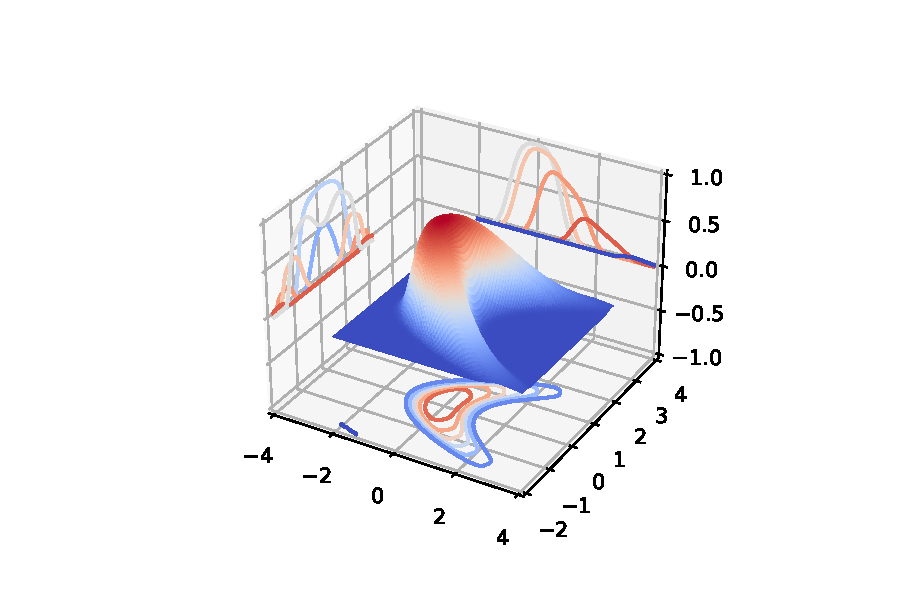
\includegraphics{Primer_figures/3dplot.pdf}
  \caption{Some descriptive text}\label{referencefigure}
\end{figure}

Figures can be included using the {\ttfamily graphicx} package. The {\ttfamily figure} environment provides some useful tools like the {\ttfamily caption} macro which allows to give a description to the figure and also referring to it using \bs{label}, check Fig.~\ref{referencefigure}, like one does with equation labels.

\section{The Minipage environment}

This environment allows you to define a box of text on which you can determine a width. The second paragraph below is within a \emph{minipage} environment.\\

Let us see how long are the lines now. ewf wefe2f we wef weof wef we we ew wef wef w wef efwef wefjwnñklwef wje fwejfw lkejlweñkjef welñk lwej lwek jelñwfj wlñke wel jwel jñlwej lñwejfl kenfwejf lñwejflwekjf wefkljwe welkjf wlkjfwlekej flwe lkwldflk weklf w\\ 

\begin{minipage}[b]{.5\textwidth}
Let us see how long are the lines now. ewf wefe2f we wef weof wef we we ew wef wef w wef efwef wefjwnñklwef wje fwejfw lkejlweñkjef welñk lwej lwek jelñwfj wlñke wel jwel jñlwej lñwejfl kenfwejf lñwejflwekjf wefkljwe welkjf wlkjfwlekej flwe lkwldflk weklf w 
\end{minipage}


\section{Defining a bibliography with `Bibtex'}

We have referenced the bibliography previously, like here \cite{Stone1932}. With \LaTeX{} one can use an automated tool to generate the bibliography, this is called `Bibtex'.  For doing it one needs to include the two statements that can be found after this paragraph. The source document needs to be parsed several times to complete the process. This is so because first one needs to know which references in the `.bib' file are cited in the document. Then a formatted bibliography file `.bbl' is created. Then the bibliography file is read and included in the document. Finally you need to run latex again to get the references properly. In summary, whenever you add some \bs{cite} references to the document you need to compile with \LaTeX{}, then `Bibtex' and then with \LaTeX{} two times again. 

% Different bibliography styles. plain, siam, abbrv, alpha

\bibliographystyle{siam}
\bibliography{my_bibliography.bib}














\end{document}














